\chapter{Data Containers}
\label{sec:datacontainer}

In this Chapter the container types available in \texttt{python} are reviewed.

\section{Lists}
\label{lists}

A list in \texttt{python} is a container that is a \emph{mutable}, ordered sequence of elements. Each element or value that is inside of a list is called an \emph{item}. Each item can be accessed using square brackets notation, \texttt{alist[index]}, where \texttt{index} is the position of the item in the list.
Remember that, list indexing is zero-based so the first element has index 0 actually. A list is considered mutable since you can add, remove or update the items in it. Ordered instead means that items are kept in the same order they have been added to. Lists can be created by enclosing in square brackets the comma-separated list of the items or using the \texttt{list()} operator.

\begin{ipython}
mylist = list([21, 32, 15])
mylist = [21, 32, 15]

print(mylist)
print (type(mylist))
\end{ipython}
\begin{ioutput}
[21, 32, 15]
<class 'list'>
\end{ioutput}

\begin{ipython}
print (mylist[0])
\end{ipython}
\begin{ioutput}
21
\end{ioutput}

If you have a list of lists (i.e. a 2-dimensional list) you can use the square brackets
multiple times to access the inner elements:
\begin{ipython}
alist = [[1,2], [3,4], [5,6]]
print (alist[1][1]) # first [1] returns [3,4], second returns 4                 
\end{ipython}  

The number of elements in a list is counted using the function \texttt{len()}:
\begin{ipython}
print(len(mylist))
\end{ipython}
\begin{ioutput}
3
\end{ioutput}

Looping on list items can be achieved in two ways: using directly the list or by index:

\begin{ipython}
print ("Loop using the list itself:")
for i in mylist:
    print (i)
\end{ipython}
\begin{ioutput}
Loop using the list itself:
21
32
15
\end{ioutput}
\begin{ipython}
print ("Loop by index:")
for i in range(len(mylist)): # len returns number of items in the list
    print (i)
\end{ipython}
\begin{ioutput}
Loop by index:
21
32
15
\end{ioutput}

With the \texttt{enumerate} function is actually possible to do both at the same time since it returns two values, the index of the item and its value, so in the example below, \texttt{i} will take the item indices while \texttt{item} the item value itself:

\begin{ipython}
for i, item in enumerate(mylist):
    print (i, item)
\end{ipython}
\begin{ioutput}
0 21
1 74
2 85
3 15
4 188
\end{ioutput}

Since a list is mutable its items can be changed dynamically:

\begin{ipython}
mylist[1] = 74 # we can change list items since it's *mutable*
print (mylist)
\end{ipython}
\begin{ioutput}
[21, 74, 15]
\end{ioutput}

With \texttt{append} an item is added at the end, while with \texttt{insert} an 
item can be added in a specified position:

\begin{ipython}
mylist.append(188) # append add an item at the end of the list
print (mylist)
\end{ipython}
\begin{ioutput}
[21, 74, 15, 188]
\end{ioutput}
\begin{ipython}
mylist.insert(2, 85) # insert an item in the desired position
                     # (2 in this example)
print (mylist)
\end{ipython}
\begin{ioutput}
[21, 74, 85, 15, 188]
\end{ioutput}

To append multiple values at once to a list a loop can be used but \texttt{python} offers a single line way of doing it: \texttt{[i*2 for i in range(10)]}. This syntax is called \emph{list comprehension}.

Accessing items outside the list range gives an error:

\begin{ipython}
mylist[10] # error ! it doesn't exists, the list has only 3
           # elements, so the last is item 2
\end{ipython}
\begin{ioutput}
Traceback (most recent call last):
  File "<stdin>", line 1, in <module>
IndexError: list index out of range
\end{ioutput}

Read carefully the error messages usually they are very explicative and can help a lot 
in \emph{debugging} (i.e. finding mistakes) in your programs.

There are two more nice features of \texttt{python} indexing:

\begin{itemize}
\tightlist
\item negative indices are like positive ones except that they starts from the last element;
\item \emph{slicing} which allows to specify a range of indices to select more items at once 
(if the first or last limits are missing slicing will start from the first or end 
with last index respectively).
\end{itemize}

\begin{ipython}
print ("negative index -1 returns the last element:", mylist[-1])
print ("slice [1:3] returns items 1st and 2nd:", mylist[0:3])
print ("slice [:2] returns items 0th and 1st:", mylist[:2])
print ("slice [2:] returns items between the 2nd and the last:", mylist[2:])
\end{ipython}
\begin{ioutput}
negative index -1 returns the last element: 188
slice [1:3] returns items 1st and 2nd: [21, 74, 85]
slice [:2] returns items 0th and 1st: [21, 74]
slice [2:] returns items between the 2nd and the last: [85, 15, 188]
\end{ioutput}
\noindent
Needless to say that slicing with \texttt{[:]} returns the entire list.

It is worth mentioning that a list doesn't have to be populated with the same kind of objects (list indices are instead always integers).

\begin{ipython}
mixedlist = [1, 2, "b", math.sqrt]
print (mixedlist)
\end{ipython}
\begin{ioutput}
[1, 2, 'b', <built-in function sqrt>]
\end{ioutput}

\begin{ipython}
print (mixedlist['k'])
\end{ipython}
\begin{ioutput}
Traceback (most recent call last):
  File "<stdin>", line 1, in <module>
TypeError: list indices must be integers or slices, not str
\end{ioutput}

A complete list of the commands available for a list can be shown with \texttt{dir(list)}:

\begin{ipython}
dir(list)
\end{ipython}
\begin{ioutput}
[...
 'append',
 'clear',
 'copy',
 'count',
 'extend',
 'index',
 'insert',
 'pop',
 'remove',
 'reverse',
 'sort']
\end{ioutput}

Their meaning is pretty clear, so for example \texttt{sort} re-order the items according to a custom criteria or \texttt{index(item)} return the index of the specified item.

\section{Dictionaries}\label{dictionaries}

A we have seen lists are ordered collections of elements and as such we can say that map integers (the index of each item) to values (any kind of \texttt{python} object). \emph{Dictionaries} generalize such a concept being containers which map \emph{keys} (\textbf{almost} any kind of \texttt{python} object) to values (any kind of \texttt{python} object).

In our previous section we had:
\[
\begin{matrix} 
0~(\textrm{0th item})& \rightarrow& 21\\
1~(\textrm{1st item})& \rightarrow& 74\\
2~(\textrm{2nd item})& \rightarrow& 85\\ 
&\cdots&  
\end{matrix}
\]
With a dictionary we can have something like this:
\[
\begin{matrix}
"apple" (\textrm{key})&\rightarrow& 4 \\
"banana" (\textrm{key})& \rightarrow& 5 \\
&\cdots&
\end{matrix}
\]
As we will see dictionaries are very flexible and will be very useful to represent complex data structures.

Dictionaries can be created by enclosing in curly brackets the comma-separated list of key-value pairs (key and value are separated by a \texttt{:} (colon)), or using the \texttt{dict()} operator. In lists we could access items by index, here we do it by key still using the square brackets. Trying to access not existing keys results in error, but we can check if a key exists with the \texttt{in} operator. As before, if a dictionary contains other dictionaries or lists, the square brackets can be applied repeatedly to access the inner items.

\begin{ipython}
adict = {"apple": 4, "banana": 5}
print (adict["apple"])
\end{ipython}
\begin{ioutput}
4
\end{ioutput}

\begin{ipython}
adict["pear"] # error !
\end{ipython}
\begin{ioutput}
Traceback (most recent call last):
  File "<stdin>", line 1, in <module>
KeyError: 'pear'
\end{ioutput}

\begin{ipython}
'pear' in adict # indeed
\end{ipython}
\begin{ioutput}
False
\end{ioutput}

The items can be dynamically created or updated with the assignment \texttt{=} operator, while again \texttt{len()} returns the number of items in a dictionary.

\begin{ipython}
adict["banana"] = 2
adict["pear"] = 10

print (len(adict))
print (adict)
\end{ipython}
\begin{ioutput}
3
{'apple': 4, 'banana': 2, 'pear': 10}
\end{ioutput}

Dictionaries can be made of more complicated types than simple string and integers:

\begin{ipython}
adict[math.log] = math.exp
\end{ipython}

Also dictionaries can be created with the \emph{comprehension} syntax: \texttt{\{i:v for i, v in enumerate(["a", "b", "c"])\}}.

Looping over dictionary items can be done by key, by value or both: \texttt{.keys()} returns a list of keys, \texttt{.values()} returns a list of values and \texttt{.items()} a list of pairs key-value.

\begin{ipython}
print ("All keys: ", adict.keys())

for key in adict.keys():
    print (key)
\end{ipython}
\begin{ioutput}
All keys:  dict_keys(['apple', 'banana', 'pear', <built-in function log>])
apple
banana
pear
<built-in function log>
\end{ioutput}
\begin{ipython}
print ("All values: ", adict.values())

for value in adict.values():
    print (value)
\end{ipython}
\begin{ioutput}
All values:  dict_values([4, 2, 10, <built-in function exp>])
4
2
10
<built-in function exp>
\end{ioutput}
\begin{ipython}
print ("All key-value pairs: ", adict.items())

for key, value in adict.items():
    print (key, value)
\end{ipython}
\begin{ioutput}
All key-value pairs:  dict_items([('apple', 4), ('banana', 2), ('pear', 10),
(<built-in function log>, <built-in function exp>)])
apple 4
banana 2
pear 10
<built-in function log> <built-in function exp>
\end{ioutput}

To merge two dictionaries the function \texttt{update()} can be used, while with \texttt{del} it is possible to remove a key-value pair.

\begin{ipython}
del adict[math.log]
seconddict = {"watermelon": 0, "strawberry": 1}
adict.update(seconddict)
print (adict)
\end{ipython}
\begin{ioutput}
{'apple': 4, 'banana': 2, 'pear': 10, 'watermelon': 0, 'strawberry': 1}
\end{ioutput}

Again the complete list of dictionary functions can be shown with \texttt{dir}:

\begin{ipython}
dir(dict)
\end{ipython}
\begin{ioutput}
[...
 'clear',
 'copy',
 'fromkeys',
 'get',
 'items',
 'keys',
 'pop',
 'popitem',
 'setdefault',
 'update',
 'values']
\end{ioutput}

\section{Tuples}\label{tuples}

Tuples create a bit of confusion for beginners because they are very similar to lists 
but they have some subtle conceptual differences, see Fig.~\ref{fig:tuples}.
Nonetheless, tuples do appear when programming in \texttt{python} so it's important to know about them.

\begin{figure}[hb]
\centering
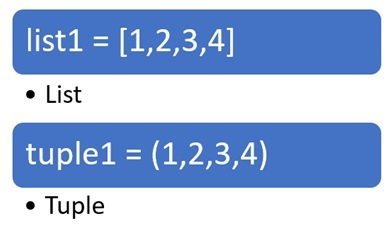
\includegraphics[width=0.5\textwidth]{figures/Difference-Between-List-and-Tuple-fig-1-2.jpg}
\caption{At first glance list and tuples look very similar, but they are not\ldots}
\label{fig:tuples}
\end{figure}

Like lists, tuples are containers of any type of object. Unlike lists though they are \emph{immutable} which means that once they have been created the content cannot be changed (i.e. no append, insert or delete of the elements). Furthermore since they are immutable they can be used as dictionary keys (lists cannot). To create a tuple the comma-separated list of items has to be enclosed in brackets, or the \texttt{tuple()} operator can be used. Accessing tuple items is done in exactly the same way as lists.

\begin{ipython}
atuple = (1, 2, 3)
print ("Length: {}".format(len(atuple)))
print ("First element: {}".format(atuple[0]))
print ("Last element: {}".format(atuple[-1]))
\end{ipython}
\begin{ioutput}
Length: 3
First element: 1
Last element: 3
\end{ioutput}

In the next snippet of code it is shown the so called unpacking which is another way to assign tuple values to variables.

\begin{ipython}
x, y, z = (10, 5, 12)
print ("coord: x={} y={} z={}".format(x, y, z))
\end{ipython}
\begin{ioutput}
coord: x=10 y=5 z=12
\end{ioutput}

If an tuple has just one element don't forget the comma at the end otherwise it will be 
treated as a single number.

\begin{ipython}
tuple2 = (1,)
print(type(tuple2))

tuple2 = (1)
print(type(tuple2))
\end{ipython}
\begin{ioutput}
<class 'tuple'>
<class 'int'>
\end{ioutput}

Since a tuple is immutable to add new elements it is necessary to create a new object:

\begin{ipython}
tuple1 = (1, 2, 3)
tuple2 = tuple1 + (4, 5)
print(tuple2)
\end{ipython}
\begin{ioutput}
(1,2,3,4,5)
\end{ioutput}

Finally, as already said tuples can be used as dictionary keys:

\begin{ipython}
d = {
	('Finance', 1): 'Room 8',
	('Finance', 2): 'Room 3',
	('Math', 1): 'Room 6',
	('Programming', 1): 'IT room'}
\end{ipython}

Below the full list of tuple functions:
\begin{ipython}
dir(dict)
\end{ipython}
\begin{ioutput}
[...
 'count',
 'index']
\end{ioutput}

\section{Exercises}
\begin{question}
What is a dictionary in \(\tt{python}\) programming language ? Create a dictionary, modify it and then print all its items.
\end{question}

\cprotEnv\begin{solution}
A dictionary is a container that maps a key (any object) to a value (any object), contrary to lists which map an integer (the index) to a value (any object).

\begin{ipython}
dictionary = {"calculus": 28, "physics":30, "chemistry":25}

dictionary["laboratory"] = 27
dictionary["chemistry"] = 24

print ("Exam\tVote")
for k, v in dictionary.items():
    print("{}:\t{}".format(k, v))
\end{ipython}
\begin{ioutput}
Exam            Vote
calculus:       28
physics:        30
chemistry:      24
laboratory:     27
\end{ioutput}
\end{solution}

\begin{question}
Write code which, given the following list 

\lstinline[language=iPython]|input\_list = [3, 5, 2, 1, 13, 5, 5, 1, 3, 4]|

\noindent
prints out the indices of every occurrence of \lstinline[language=iPython]|y=5|.
\end{question}

\cprotEnv\begin{solution}
\begin{ipython}
l = [3, 5, 2, 1, 13, 5, 5, 1, 3, 4]

for i in range(len(l)):
    if l[i] == y:
        print (i)
\end{ipython}
\begin{ioutput}
1
5
6
\end{ioutput}
Note that lists already have a way to get the occurrences of an item: \texttt{l.count(5)} would have done the job.
\end{solution}

\begin{question}
Write a \texttt{python} program to convert a list of tuples into a dictionary where the keys are the first elements of each tuples and the values the second.

\noindent
Input: \lstinline[language=iPython]|l = [("x", 1), ("x", 2), ("x", 3), ("y", 1), ("y", 2), ("z", 1)]|
\end{question}

\cprotEnv\begin{solution}
\begin{ipython}
l = [("x", 1), ("x", 2), ("x", 3), ("y", 1), ("y", 2), ("z", 1)]

d = {}
for item in l:
    d[item][0]] = item[1]
    
print(d)
\end{ipython}
\begin{ioutput}
{'x': 3, 'y': 2, 'z': 1}
\end{ioutput}
Note that there is just one occurrence of the key $\tt{x}$ and $\tt{y}$ because keys has to be unique and setting the same key to a different value simply overwrite the existing entry.
\end{solution}

\begin{question}
Write a \texttt{python} program to increment by 10 the last value of each tuples in a list.

\noindent
Input: \lstinline[language=iPython]|l = [(10, 20, 40), (40, 50, 60), (70, 80, 90)]|.
\end{question}

\cprotEnv\begin{solution}
\begin{ipython}
l = [(10, 20, 40), (40, 50, 60), (70, 80, 90)]

for i in range(len(l)):
    new_tuple = l[:-1] + [l[2] + 10]
    l[i] = new_tuple
    
print (l)
\end{ipython}
\begin{ioutput}
[(10, 20, 50), (40, 50, 70), (70, 80, 100)]
\end{ioutput}
\end{solution}

\begin{question}
Write a \texttt{python} program to count the elements in a list until an element is a tuple.

\noindent
Input:\lstinline[language=iPython]|l = [1, 5, 'a', (1, 2), 'test':1]|
\end{question}

\cprotEnv\begin{solution}
\begin{ipython}
l = [1, 5, 'a', (1, 2), 'test':1]

number_of_items = 0 
for item in l:
    if type(item) != 'tuple'{:}
        number_of_items += 1
    else:
        break
        
print("There are {} items before a tuple.".format(number_of_items))
\end{ipython}
\begin{ioutput}
\end{ioutput}
\end{solution}

\begin{question}
Write a \texttt{python} script to concatenate the following dictionaries to create a new single one.

\noindent 
Input:
\lstinline[language=iPython]|dic1 = \{1:10, 2:20\}; dic2 = \{3:30, 4:40\}; dic3 = \{5:50, 6:60\}|
\end{question}

\cprotEnv\begin{solution}
\begin{ipython}
dic1 = {1:10, 2:20}
dic2 = {3:30, 4:40}
dic3 = {5:50, 6:60}

dic_tot = dict()
dic_tot.update(dic1)
dic_tot.update(dic2)
dic_tot.update(dic3)

print(dic_tot)
\end{ipython}
\begin{ioutput}
{1: 10, 2: 20, 3: 30, 4: 40, 5: 50, 6: 60}
\end{ioutput}

An alternative and even more concise way using the \texttt{**} operator is the following:
\begin{ipython}
dic1 = {1:10, 2:20}
dic2 = {3:30, 4:40}
dic3 = {5:50, 6:60}

new_dic = {**dic1, **dic2, **dic3}
\end{ipython}
\end{solution}

\begin{question}
Write a \texttt{python} script to check whether a given key already exists in a dictionary.
\end{question}

\cprotEnv\begin{solution}
\begin{ipython}
dic = {"a":1, "b":2, "c":3}

print("z" in dic)
print("a" in dic)
\end{ipython}
\begin{ioutput}
False
True
\end{ioutput}
\end{solution}

\begin{question}
Write a \texttt{python} program to combine two dictionary adding values for common keys.

\noindent
Input: \lstinline[language=iPython]|d1 = \{'a':100, 'b':200, 'c':300\}; d2 = \{'a':300, 'b':200, 'd':400\}|
\end{question}

\cprotEnv\begin{solution}
\begin{ipython}
d1 = {'a':100, 'b':200, 'c':300}
d2 = {'a':300, 'b':200, 'd':400}

d = {}
d.update(d1)

for k in d2.keys():
    if k in d:
        d[k] = d[k] + d2[k]
    else:
        d[k] = d2[k]

print(d)
\end{ipython}
\begin{ioutput}
{'a': 400, 'b': 400, 'c': 300, 'd': 400}
\end{ioutput}
\end{solution}

\begin{question}
Given the following dictionary mapping currencies to 2-year zero coupon bond prices, build another dictionary mapping the same currencies to the corresponding annualized interest rates.

\lstinline[language=iPython]|d = {'EUR':0.9, 'CHF':1.005, 'USD':0.985, 'GBP':0.97}|
\end{question}

\cprotEnv\begin{solution}
The price of a n-years zero coupon bond is:

\[ P = \frac{M}{(1+r)^{n}} = M\cdot D \]
where $M$ is the value of the bond at the maturity, $r$ is the risk-free rate and $n$ is the number of years until maturity.
%Hence:

\[ D = \cfrac{1}{(1+r)^{n}} \implies r = \Big(\cfrac{1}{D}\Big)^{\cfrac{1}{n}} - 1\]

\begin{ipython}
# initialize an empty dictionary in which to store result
rates = {}

maturity = 2
discount_factors = {'EUR':0.9, 'CHF':1.005, 'USD':0.985, 'GBP':0.97}

# loop over the input dictionary to get the currencies
for currency, df in discount_factors.items():
    # calculate the rate and store it in the output dictionary
    rates[currency] = pow(1/df, 1/maturity) - 1
   
for r in rates.items():
    print(r)
\end{ipython}
\begin{ioutput}
('EUR', 0.05409255338945984)
('CHF', -0.002490663892367073)
('USD', 0.007585443719756668)
('GBP', 0.015346165133619083)
\end{ioutput}
\end{solution}

\begin{thebibliography}{9}
\bibitem{lists} \href{https://docs.python.org/3/tutorial/datastructures.html}{\emph{Data Structures, More on Lists}} [Online]
\bibitem{dictionaries} \href{https://realpython.com/python-dicts/}{\emph{Dictionaries in Python}}, Real Python [Online]
\bibitem{tuple} \href{https://www.programmareinpython.it/video-corso-python-base/14-liste-e-tuple/}{\emph{Liste e Tuple}}, Programmare in Python [Online]
\end{thebibliography}

